\documentclass{bachelor_report}

% Додаткові пакети вносіть у цей файл
\usepackage{euscript}
\usepackage{xcolor}


% Додаткові визначення та перевизначення кось лінк на оверліфось лінк на оверліфоманд вносіть у цей файл
%%% Ó äàíîìó ôàéë³ âèçíà÷àéòå âñ³ íåîáõ³äí³ âàì íîâ³ êîìàíäè TeX
%%% àáî ðîá³òü ïåðåâèçíà÷åííÿ ³ñíóþ÷èõ, íàïðèêëàä...

% Ïåðåâèçíà÷åííÿ ñèìâîëó ïîðîæíüî¿ ìíîæèíè òà çíàê³â "á³ëüøå-äîð³âíþº", "ìåíøå-äîð³âíþº" íà ïðèéíÿò³ ó íàñ
\let\oldemptyset\emptyset
\let\emptyset\varnothing
\let\geq\geqslant
\let\leq\leqslant

% Âèçíà÷åííÿ íîâèõ ìàòåìàòè÷íèõ êîìàíä
\newcommand*{\binsp}[1]{\ensuremath \left\{0, 1\right\}^{#1}}       % {0, 1}^m
\newcommand*{\xor}{\ensuremath \oplus}                              % \xor = (+)
\newcommand*{\GF}[1]{\ensuremath \mathbb F_{#1}}                    % F_n
\newcommand*{\GFgroup}[1]{\ensuremath \mathbb F^{*}_{#1}}           % F^*_n
\newcommand*{\Zring}[1]{\ensuremath \mathbb Z_{#1}}                 % Z_n
\newcommand*{\Zgroup}[1]{\ensuremath \mathbb Z^{*}_{#1}}            % Z^*_n
\newcommand*{\Jset}[1]{\ensuremath \mathbb J_{#1}}                  % J_n
\newcommand*{\Qset}[1]{\ensuremath \mathbb Q_{#1}}                  % Q_n
\newcommand*{\PQset}[1]{\ensuremath \widetilde{\mathbb Q}_{#1}}     % Q~_n
\newcommand*{\cyclic}[1]{\ensuremath \left\langle {#1} \right\rangle}                  % <g>
\newcommand*{\Legendre}[2]{\ensuremath \left( \frac{#1}{#2} \right)}  % ñèìâîë Ëåæàíäðà/ßêîáè
\newcommand*{\compinv}[1]{\ensuremath {#1}^{\left\langle -1 \right\rangle}}  % îáðàòíûé ïî êîìïîçèöèè

% ²íøèé ñïîñ³á âèçíà÷åííÿ ìàòåìàòè÷íîãî îïåðàòîðó
\DeclareMathOperator{\ord}{ord}
\DeclareMathOperator{\lcm}{lcm}
\DeclareMathOperator{\Li}{Li}
\DeclareMathOperator{\Coef}{Coef}
\DeclareMathOperator{\Log}{Log}
\DeclareMathOperator{\Exp}{Exp}
\DeclareMathOperator{\Res}{Res}
\DeclareMathOperator{\charact}{char}
\DeclareMathOperator{\Sym}{Sym}

%%% ...³ òàêå ³íøå

% Відомості про автора роботи
%%% Основные сведения %%%
\newcommand{\reportAuthor}
{Дідух Максим Андрійович}
\newcommand{\reportAuthorGroup}
{ФІ-13}
\newcommand{\reportTitle}
{Назва дослідження}
%% використовуйте символ "\par" або "\\" для розбиття назви на декілька рядків


\newcommand{\supervisorFio}
{Кучинська Наталія Вікторівна}
\newcommand{\supervisorRegalia}
{кандидат технічних наук, доцент}

% Починаємо верстку документа
\begin{document}

\setfontsize{14}

% Створюємо титульну сторінку
\thispagestyle{empty}

\begin{center}
НАЦІОНАЛЬНИЙ ТЕХНІЧНИЙ УНІВЕРСИТЕТ УКРАЇНИ \par
<<КИЇВСЬКИЙ ПОЛІТЕХНІЧНИЙ ІНСТИТУТ ім. Ігоря СІКОРСЬКОГО>>\par
НАВЧАЛЬНО-НАУКОВИЙ ФІЗИКО-ТЕХНІЧНИЙ ІНСТИТУТ\par

\vspace{40mm}
{\huge Звіт з виконання кваліфікаційного дослідження \par}

\huge\MakeUppercase{\textbf{\reportTitle}} \par
\end{center}

\vspace{40mm}
\begin{flushright}
Виконав студент

групи \reportAuthorGroup

\reportAuthor

\vspace{20mm}
Науковий керівник:

\supervisorRegalia

\supervisorFio

\end{flushright}

\vspace{20mm}
\begin{center}
{Київ~--- 2025}
\end{center}

\newpage
\thispagestyle{plain}


\pagestyle{fancy}
\fancyhf{}
\fancyhead[R]{\thepage}
\renewcommand{\headrulewidth}{0pt}
\renewcommand{\footrulewidth}{0pt}

%% Створюємо зміст    % -- розкоментуйте, якщо зміст вам потрібен
\pagenumbering{gobble}
\tableofcontents
\cleardoublepage
\pagenumbering{arabic}

\setcounter{page}{2}    %!!! -- продумати, як автоматизувати номер сторінки

%% Якщо ви використовуєте зміст, то прослідкуйте, щоб номер сторінки 
%% співпадав із справжнім!

% Створюємо перелік умовних позначень, скорочень і термінів
% Якщо цей розділ вам не потрібен, просто закоментуйте два наступних рядка
\shortings
%!TEX root = ../thesis.tex
ШІ --- штучний інтелект

NIST - Національний інститут стандартів і технологій США (англ. U.S. National Institute of Standards and Technology)

RSA --- асиметрична криптосистема запропонована Рівестом, Шаміром та Адлеманом (англ. Rivest-Shamir-Adelman) у 1977 р.

AES --- покращений стандарт шифрування (англ. Advanced Encryption Standard) опублікований NIST  у 2001 р.

ГПВЧ --- генератор псевдовипадкових чисел

PCFG --- імовірнісна контекстно-вільна граматика (англ. Probabilistic Context-Free Grammar)

LSTM --- довга короткочасна пам'ятть (англ. Long short-term memory)

LSTM-мережі --- мережі з довгою короткочасною пам'яттю

GAN --- генеративна змагальна мережа (англ. Generative Adversarial Network)

PassGAN --- реалізація GAN мережі для задачі вгадування паролів (англ. Password Generative Adversarial Network)

GNPassGAN --- реалізація GAN мережі для задачі вгадування паролів з використанням градієнтної нормалізації (англ. Gradient Normalization Password Generative Adversarial Network)

Char10 --- паролі довжини до 10 симолів (англ. Characters 10)

Char812 --- паролі довжини від 8 до 12 симолів (англ. Characters 8-12)

FG --- згенерований файл паролів (англ. generated password file)

FT --- тестовний файл паролів (англ. testing password file)

% Створюємо вступ
\intro
%!TEX root = ../thesis.tex
\textcolor{red}{todo}

\textbf{Актуальність дослідження ...}

\textbf{Метою дослідження є ...}

\textbf{Задача дослідження ...}

\textbf{Об'єктом дослідження є ...}

\textbf{Предметом дослідження є ...}

\textbf{Наукова новизна ...}

\textbf{Практичне значення ...}

\textbf{Апробація результатів та публікації ...}



% Додаємо глави
% Якщо ваша робота містить менше або більше глав - модифікуйте наступні 
% рядки відповідним чином
\chapter{Застосування штучного інтелекту в криптографії, }
\label{chap:review}
У першому розділі даної роботи ми розглянемо застосування штучного інтелекту в криптографії. Дослідимо задачу вгадування паролів через, розглянемо різні підходи до її вирішення - як імовірнісні моделі (включаючи марковські моделі та PCFG), так і моделі на основі глибинного навчання. Особливу увагу приділимо GNPassGAN, розглянемо огляд GAN мереж, їх типові випадки використання, та детально порівняємо реалізації PassGAN та GNPassGAN через аналіз експериментів, метрик та їх порівняння.

% фігня)))
% \section{Коротко про АІ}  
% Штучний інтелект (ШІ) - це технологія, яка покращує різні аспекти нашого повсякденного життя. Його застосування варіюється від прогнозування погоди і навігації до класифікації зображень і відео, а також автоматизованої генерації коду, тексту і відеоконтенту.

% Вплив штучного інтелекту поширюється і на інші важливі технологічні сфери, зокрема, на блокчейн і кібербезпеку. Криптографія, яка є фундаментальним компонентом як у системах блокчейн, так і в системах кібербезпеки, може бути значно покращена завдяки інтеграції ШІ для посилення захисту приватності та підтримки цілісності.

% \section{Коротко про крипту}  
% Криптографія займається захистом інфорації та повідомлень, що передається через відкритий канал в пристуності зловмисників. Вона дозволяє лише одержувачу повідомлень переглядати її вміст. \textcolor{red}{?Широкозастосовна?} у всіх сферах, де конфіденційність та цілісність даних має значення. Використовується два види криптографічних систем: симетрична та асиметрична. У симетричній криптографії для шифрування та дефишрування даних використовується один і той же секретний ключ. В асиметричній криптографії ж використовується пара ключів - публічний та приватний. Публічний ключ відомий всім користувачам мережі, приватний ключ відомий лише одному користувачу - його власнику. Загалом, ці два ключі пов'язані між собою якимось математичним співвідношенням, яке робить неможливим визначення секретного ключа знаючи лише відкритий. Для шифрування повідомлення, відправник шифрує повідомлення використовуючи відкритий ключ одержувача, одержувач дешифрує отримане повідомення використовуючи свій приватний ключ. Криптоаналіз - процес вивчення криптографічних систем на предмет вразливості. 

% \begin{definition}
% Принцип Кірхгофа - специфікація алгоритмів шифрування та дешифрування вважається відкритою. Єдиною секретною інформацією є ключ. 
% \end{definition}

\section{Використання штучного інтелекту в криптографії}
\subsection{Штучний інтелект та еволюційні обчислення для генерування алгоритмів шифрування}
Наукова робота \cite{Cryptography using Artificial Intelligence Jonathan Blackledge} представляє інноваційний підхід до шифрування з використанням нейронних мереж та еволюційних обчислень. Автори пропонують метод, який відходить від традиційних підходів до шифрування, генеруючи персоналізовані алгоритми шифрування, а не просто використовуючи персональні ключі з відомими алгоритмами.

Основна концепція полягає у використанні природних джерел шуму, таких як атмосферний шум від радіовипромінювання та радіоактивного розпаду, для навчання систем, які можуть генерувати унікальні алгоритми шифрування. Процес починається з подачі цих природних джерел шуму в систему, яка потім вчиться апроксимувати вхідний шум для створення нелінійних функцій. Ці функції згодом використовуються як ітератори і проходять ретельне тестування на криптографічну стійкість, включаючи перевірку на показники Ляпунова, рівні ентропії, довжину циклу і характеристики дифузії ключа.

Що робить цей підхід особливо цінним, так це його здатність генерувати необмежену кількість унікальних генераторів псевдовипадкових чисел (ГПВЧ), які можуть бути використані на індивідуальній основі. Це особливо актуально для сучасних додатків, таких як безпечні хмарні сховища, де користувачі можуть отримати персоналізовані алгоритми шифрування, а не покладатися на стандартні алгоритми, які можуть бути вразливими до відомих алгоритмічних атак.


Дослідження є значним \textcolor{blue}{(а він точно значний?)))} кроком вперед у галузі криптографії, пропонуючи новий спосіб підвищення безпеки даних завдяки застосуванню штучного інтелекту.

\subsection{Нейронні мережі у криптографії}
У статті\cite{Applications of Neural Network-Based AI in Cryptography}, автор досліджує використання нейронних мереж в класичних криптографічних системах, зокрема RSA і AES. Оскільки дослідники продовжують вивчати нові підходи, штучний інтелект став цінним інструментом у розумінні та оцінці цих криптографічних стандартів.

У криптографічній системі RSA штучний інтелект і нейронні мережі продемонстрували неабиякий потенціал у кількох ключових сферах. Нейронні мережі можна навчити розпізнавати складні шаблони в процесах генерації ключів RSA, потенційно виявляючи слабкі місця, які традиційний аналіз може пропустити. Наприклад моделі глибинного навчання можуть аналізувати великі масиви даних ключів RSA для виявлення статистичних закономірностей і потенційних вразливостей в алгоритмах генерації ключів. Алгоритми машинного навчання продемонстрували успіх в оптимізації вибору і реалізації параметрів RSA, що потенційно підвищує безпеку і продуктивність. Підходи на основі штучного інтелекту навіть почали кидати виклик деяким традиційним припущенням про безпеку ключів RSA.

Штучний інтелект також відкриває нові підходи до криптоаналізу алгоритмів симетричного шифрування, тут будуть згадані тільки деякі результати для алгоритму AES, але слід зазначити, що аналогічні результит можна отримати і для інших алгоритмів. Нейронні мережі успішно застосовуються для аналізу процесів шифрування та дешифрування, намагаючись виявити тонкі закономірності або слабкі місця, які можуть бути використані. Методи машинного навчання виявилися особливо цінними при проведенні атак побічних каналів, коли системи штучного інтелекту аналізують найдрібніші зміни в енергоспоживанні, електромагнітних випромінюваннях і хронометражі під час операцій шифрування. Ці підходи показали багатообіцяючі результати в прогнозуванні ключових бітів AES і підтримці ширших криптоаналітичних зусиль. Дослідники також розробили моделі штучного інтелекту, здатні аналізувати статистичні властивості операцій AES, потенційно виявляючи раніше невідомі вразливості. Застосування глибинного навчання для диференціального та лінійного криптоаналізу AES відкрило нові шляхи для розуміння властивостей безпеки шифру.

Хоча штучний інтелект продемонстрував значний потенціал у криптографічному аналізі, наразі він слугує скоріше додатковим інструментом, ніж заміною традиційним методам. Подальший розвиток методів штучного інтелекту в криптографії відкриває нові можливості для майбутніх досліджень і розробок.

\section{\textcolor{blue}{означення геш функцій, ???мд5 геш функції???}}

\section{Задача вгадування паролів, основні підходи до її вирішення}  
Паролі є найбільш поширешим способом аутентифікації, імовірніше за все, через те, що їх легко запам'ятати та реалізувати. Незважаючи на цінність даних, доступ до яких надає кожен конкретний пароль, середньостатистичний користувач все ще використовує відносно прості паролі, що мають семантичний зміст та легко запам'ятовуються. Все це робить користувацькі паролі все більш вразливими до загроз реального світу. Посилаючись на дослідження Пірмана \cite{Observing passwords in their natural habitat}, 40\% користувачів використовують один і той же пароль на декількох різних платформах. Існує велика кількість різних технік для вгадування паролів, всі вони націлюються на взлам як можна більшої кількості паролів за найменшу кількість спроб. Виділяють два основних типи атак - онлайн та оффлайн. 

\begin{definition}
Оффлайн атака - атака під час якої, атакуючий якимось чином отримати певну кількість криптографічних гешів паролів користувачів та намагається відновити їх вгадуючи та тестуючи велику кількість паролів.
\end{definition}

\begin{definition}
Онлайн атака - атака під час якої, атакуючий робить спроби вгадати пароль через web-інтерфейс або додаток.
\end{definition}

\begin{remark}
Слід зазначити, що онлайн атаки є більше обмеженими тому, що більшість web-інтерфейсів та додатків, обмежують можливість надсилання запитів після певної кількості невдалих спроб. Таких обмежень не може бути у випадку оффлайн атак, де атакуючи ніяк не взаємодіє з іншими сервісам, виконуючи вгадування в ізольованому середовищі.
\end{remark}

До того ж існують й інші властивості атак, які визначають кількість інформації про користувача, що має атакуючий. Тут також є два основних типи - тралення (англ. trawling) та націлене вгадування.

\begin{definition}
Націлене вгадування виникає тоді, коли атакуючий намагається дізнатись пароль користувача використовуючи будь-які дані, що мають відношення до конкретного користувача.    
\end{definition}

Ванг \cite{Targeted online password guessing} запропонував класифікувати таку інформацію на дві категорії в залежності від ступеня конфіденційності. Перший тип - це особиста інформація користувача, що надає змогу ідентифікувати його, включаючи ім'я, електронну пошту, тощо. Другий тип - це ідентифікаційні дані користувача, які є частково публічними (наприклад, ім'я користувача) і частково приватними (наприклад, пароль).

\begin{definition}
Тралення (англ. trawling) - атака, під час якої, атакуючий намагається знайти користувача, що відповідає уже відомому паролю.
\end{definition}

\begin{remark}
Більшість користувачів не заслуговують націлених атак, як правило кількість ресурсів які атакуючий витратить на націлену атаку перевищить кількість ресурсів, які він отримає після успішного взламу. Сконцентрованої уваги заслуговують лише спеціальні користувачі, що \textcolor{blue}{відносятся?} стосуються критичної інфраструктури, фінансових установ або документів.
\end{remark}

Далі наведені деякі з відомих типів атак. Слід зазначити, що всі вони використовують \textcolor{blue}{норм лишити англ?} trawling offline guessing , коли атакуючий якимось чином здобув доступ до бази даних, що містить геші паролів.

\section{\textcolor{blue}{Моделі що базуються на правилах?} Rule-based моделі}
На просторах мережі Інтернет можна зайти величезну кількість викрадених паролів, ось найбільші з них \cite{GNPassGAN: Improved Generative Adversarial Networks For Trawling Offline Password Guessing}:

\begin{table}[h]
\centering
\begin{tabular}{|l|c|}
\hline
\textbf{Джерело} & \textbf{К-ть паролів} \\
\hline
phpBB & $3.0 \times 10^5$ \\
Yahoo & $4.4 \times 10^5$ \\
Rock You & $1.4 \times 10^7$ \\
Myspace & $5.5 \times 10^4$ \\
SkullSecurityComp & $6.7 \times 10^6$ \\
LinkedIn & $1.3 \times 10^6$ \\
\hline
\end{tabular}
\caption{Відомі відкриті бази паролів}
\end{table}

Велика кількість викрадених паролів справжніх користувачів сильно спрощує вивчення та збір патернів паролів. Маючи таку велику вибірку можна створити нові паролі-кандидати, використовуючи наявні як приклад. Прикладами таких реалізацій є John The Ripper3\footnote{https://github.com/openwall/john} та Hashcat 2\footnote{https://github.com/hashcat/hashcat}, ці програми реалізують велику варіативність методів взламу паролів, таких як прямий перебір, атаки з використанням словників та \textcolor{blue}{норм лишити англ?} rule-based атак, яка є найшвидшою серед усіх атак. 

\begin{remark}
\textcolor{blue}{норм лишити англ?} Rule-based системи генерують паролі виключно базуючись на вже відомих правилах, а створення нових правил є складною задачею, що вимагає великого рівня експертизи. 
\end{remark}

\begin{corollary}
\textcolor{blue}{чи потрібно виносити це як наслідок?} Паролі, для яких складно побудувати правила будуть взламуватись набагато важче, якщо будуть взагалі.
\end{corollary}

\section{Імовірністі моделі}
Імовірнісні моделі представляють собою фундаментальний клас методів для аналізу та генерації паролів, що базуються на статистичних закономірностях у навчальних даних. Ці моделі використовують математичний апарат теорії ймовірностей для оцінки вірогідності появи певних послідовностей символів у паролях. На відміну від простих словникових атак, імовірнісні моделі здатні генерувати нові паролі, які не містяться в навчальному наборі, але відповідають статистичним патернам реальних паролів. Далі ми розглянемо два основних підходи: марковські моделі, що базуються на послідовних залежностях між символами, та моделі на основі імовірнісних контекстно-вільних граматик (PCFG), які враховують структурні особливості паролів. Обидва підходи мають свої переваги та обмеження, і їх розуміння є критичним для подальшого розвитку методів аналізу паролів.

\subsection{Марковська модель}
Марковська модель являє собою фундаментальний підхід до підбору паролів, що походить від принципів мовного моделювання та була представлена Нараньяном \cite{Fast dictionary attacks on passwords using timespace tradeoff}. Ця модель передбачає наступні символи в послідовності на основі попередніх символів, причому довжина контексту, відома як «порядок», відіграє вирішальну роль в її ефективності. Еволюція моделі зазнала значних покращень завдяки дослідженням Ма \cite{A study of probabilistic password models}, які запровадили складні методи, такі як нормалізація кінцевих символів та згладжування Лапласа. Нормалізація кінцевих символів працює шляхом додавання певного символу до паролів, гарантуючи, що розподіли ймовірностей зберігають математичну узгодженість. Згладжування за Лапласом вирішує критичну проблему надмірної підгонки шляхом введення дельта-значення до підрахунку підрядків, що особливо корисно для марковських моделей вищих порядків, які обробляють більш обширну контекстну інформацію.

\subsection{Модель PCFG}
Модель на основі імовірнісних контекстно-вільних граматик (PCFG), представлена Вейром \cite{Password cracking using probabilistic context-free grammars} у 2009 році, являє собою складний підхід до аналізу паролів за допомогою структурної декомпозиції. Ця модель ґрунтується на фундаментальній передумові, що паролі можна розбити на незалежні шаблонні структури, кожна з яких містить окремі термінали. Модель обчислює ймовірності паролів шляхом множення ймовірностей структур і відповідних їм терміналів. Наприклад, пароль типу «rockyou123» аналізується шляхом розбиття його на окремі структури («L7» для літер і «D3» для цифр) і відповідні їм закінчення («rockyou» і «123»). Можливості моделі було значно розширено завдяки кільком інноваціям, включаючи інтеграцію піньїнь\footnote{Піньїнь, повна офіційна назва Ханьюй піньїнь — найпоширеніший стандарт латинізування китайської мови, тобто позначення звуків китайської за допомогою латинської абетки.\cite{Pinyin wiki}} для аналізу китайських паролів у роботі Лі \cite{A large-scale empirical analysis of chinese web passwords}, а також включення шаблонів клавіатури та багатослівних шаблонів \cite{Next gen pcfg password crackingt}. Ма \cite{A study of probabilistic password models} продемонстрував підвищену точність вгадування, проаналізувавши шаблони кінцевих частот у навчальних даних.

\section{Моделі глибинного навчання}
На відміну від \textcolor{blue}{норм лишити англ?} rule-based та імовірнісних моделей вгадування паролів, методи глибинного навчання не роблять жодних припущень щодо структури паролів. Множини паролів згенеровані таким методом не обмежуються лише певною підмножиною відомих паролів.

Нейронні мережі, особливо мережі з довгою короткочасною пам'яттю (LSTM-мережі) \cite{Long short-term memory}, представляють собою передову технологію підбору паролів. Ці мережі є обчислювальними моделями, які імітують біологічні нейронні мережі, пропонуючи складні можливості апроксимації функцій. Нейромережевий підхід долає суттєве обмеження марковських моделей - обмеження контексту фіксованої довжини - шляхом збереження довгострокових залежностей у даних. Меліхер \cite{Fast lean and accurate: Modeling password guessability using neural networks} вперше застосував цей підхід, використовуючи LSTM-мережі для вилучення та прогнозування ознак паролів, хоча їхня оцінка була \textcolor{blue}{обмежена обмеженими} обмежена обмеженими структурами та даними \cite{Regularizing and optimizing lstm language models}. З тих пір ця область розвивалася за допомогою різних нових підходів, включаючи впровадження Хітай \cite{Passgan: A deep learning approach for password guessing} генеративних змагальних мереж (GAN) для вгадування паролів, хоча це вимагало більше спроб вгадування, ніж моделі на основі LSTM. Лю \cite{Genpass: A general deep learning model for password guessing with pcfg rules and adversarial generation} пішли далі, створивши гібридний підхід, який поєднав правила PCFG з LSTM-мережами, показавши значні покращення. Однак їхнє тестування було обмежене \(10^{12}\) вгадуваннями, тоді як реальні сценарії тралення в автономному режимі часто вимагають до \(10^{16}\) спроб. Сюй \cite{Password guessing based on lstm recurrent neural networks} також реалізував мережі LSTM, але обмежив їх оцінку до \(10^{10}\) вгадувань, не проводячи комплексної оцінки.

\section{GNPassGAN: Покращена генеративна мережа для підбору паролів в оффлайн режимі}
Тепер розглянемо новий підхід до вгадування паролів з використанням вдосконалених генеративних змагальних мереж. GNPassGAN представляє собою значний крок вперед у застосуванні глибинного навчання для аналізу та генерації паролів, пропонуючи покращену архітектуру в порівнянні з попередніми підходами. Ми детально розглянемо теоретичні основи генеративних змагальних мереж (GANs), їх практичне застосування в різних областях, а також специфіку їх адаптації для задачі вгадування паролів. Особливу увагу буде приділено порівняльному аналізу PassGAN та його вдосконаленої версії GNPassGAN, включаючи детальний розбір експериментальних результатів та метрик ефективності. Цей розділ надасть комплексне розуміння того, як сучасні методи машинного навчання можуть бути ефективно застосовані для вирішення складних задач у сфері криптографії та кібербезпеки.

\subsection{Огляд генеративних змагальних мереж}
Генеративні змагальні мережі (GAN), представлені Гудфеллоу у 2014 році \cite{Goodfellow GANs NIPS}, представляють новий підхід до генеративного моделювання з використанням глибинного навчання. Архітектура реалізує змагальну структуру, де дві нейронні мережі змагаються одна проти одної в грі на мінімакс\footnote{Мінімакс (англ. minimax, нім. minimax n) — правило прийняття рішень, що використовується в теорії ігор, теорії прийняття рішень, дослідженні операцій, статистиці і філософії для мінімізації можливих втрат з тих, які особа, яка приймає рішення не може уникнути при розвитку подій за найгіршим для неї сценарієм.\cite{minimax wiki}}. Перша мережа, відома як Генератор (G), створює синтетичні дані, намагаючись імітувати реальний розподіл даних, тоді як друга мережа, Дискримінатор (D), має на меті розрізняти реальні та згенеровані дані.

Фундаментальна робота GAN полягає в тому, що Генератор приймає випадковий шум з латентного простору як вхідний сигнал і виробляє синтетичні зразки. Одночасно Дискримінатор функціонує як \textcolor{blue}{(розписати більше про дискримінатор, генератор та двійковий класифікатор?)} двійковий класифікатор, виводячи ймовірність того, що будь-який вхідний сигнал є справжнім, а не згенерованим. Завдяки цьому змагальному процесу навчання, обидві мережі постійно вдосконалюють свої можливості: Генератор покращує свою здатність створювати більш переконливі синтетичні дані, тоді як Дискримінатор вдосконалюється у їх виявленні.

\subsection{Поширені випадки використання GAN мереж}
GAN мережі знайшли застосування у різних галузях. У сфері комп'ютерного зору такі архітектури, як StyleGAN \cite{StyleGAN}, зробили революцію у створенні синтетичних зображень, створюючи фотореалістичні людські обличчя, які неможливо відрізнити від справжніх фотографій. Медична галузь використовує GANs для створення синтетичних даних медичних зображень, вирішення проблем конфіденційності та доповнення обмежених наборів даних для рідкісних захворювань.

Ще одним значним проривом стало перетворення тексту в зображення: такі моделі, як DALL-E\footnote{https://openai.com/index/dall-e/} і Stable Diffusion\footnote{https://stabledifffusion.com/}, використовують архітектуру, натхненну GAN, для створення зображень з текстових описів. В аудіо області GAN дозволили синтезувати голос і створювати музику, в той час як в обробці відео вони сприяли прогнозуванню кадрів і поліпшенню якості відео \cite{Video to video synthesis}.

\begin{figure}[ht]
        \centering
        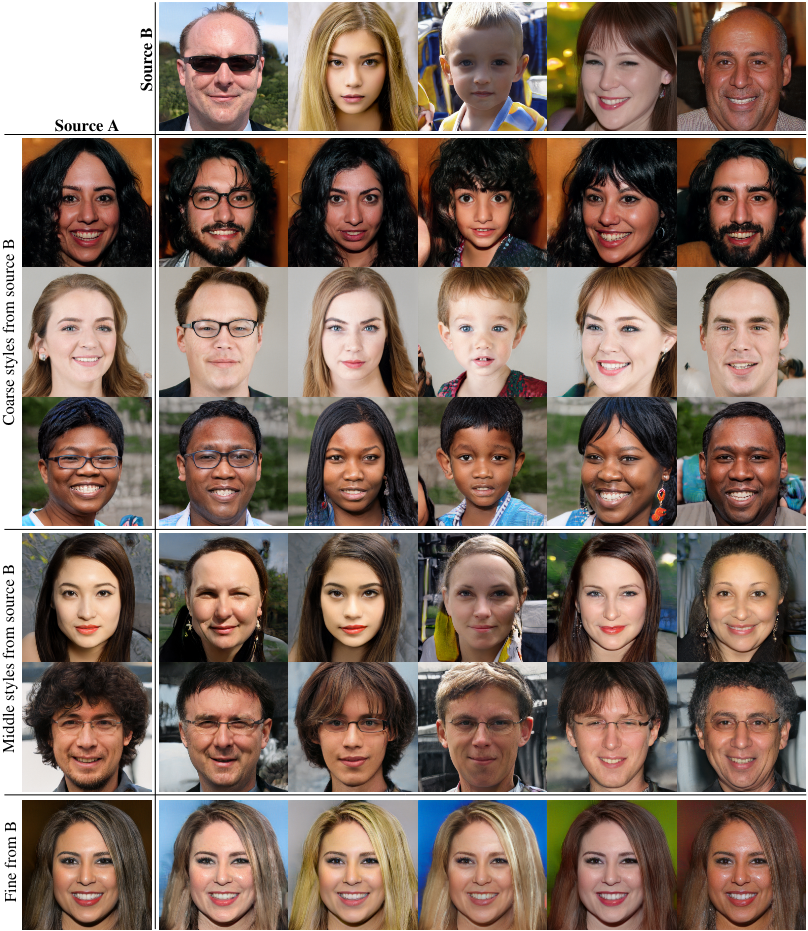
\includegraphics[scale=0.4]{Images/GAN_generated_image.png}
        \caption{\textcolor{red}{fix caption} image from here: https://arxiv.org/pdf/1812.04948}
        \label{gan_generated_image}
\end{figure}
\newpage

\subsection{Реалізації GAN мереж для вирішення задачі вгадування паролів, PassGAN та GNPassGAN}
\textcolor{red}{я б хотів бачити детальніший опис структур цих двох реалізацій, та їх різницю, чому одне краще за інше}
Застосування генеративних змагальних мереж для вгадування паролів відкрило новий напрямок у розвитку методів тестування безпеки паролів. На відміну від традиційних підходів, таких як словникові атаки чи правила трансформації, GAN мережі здатні вивчати та відтворювати складні патерни в реальних паролях, генеруючи при цьому нові, потенційно валідні комбінації. Це особливо важливо в контексті сучасних вимог до безпеки, де паролі стають все складнішими та різноманітнішими. Розглянемо дві ключові реалізації цього підходу, які демонструють еволюцію застосування GAN у сфері аналізу паролів.

PassGAN - це генеративна змагальна мережа, призначена для підбору паролів, запропонована Хітаджем \cite{Passgan: A deep learning approach for password guessing}. Це було одне з перших застосувань GAN для вирішення задачі вгадування паролів. Модель використовує традиційну архітектуру GAN, де генератор і дискримінатор змагаються в мінімаксній грі для двох гравців. PassGAN була протестована на паролях з довжиною менше 10 символів і показала потенціал глибинного навчання для генерації паролів.

GNPassGAN є покращеною версією PassGAN, яка вводить кілька ключових архітектурних модифікацій для покращення можливостей генерації паролів. Модель зберігає базову структуру GAN, але впроваджує важливі зміни для підвищення стабільності та продуктивності. Як ми побачимо далі, GNPassGAN має кращі результати, тому це й буде основним предметом дослідження в даній роботі. 

\subsection{Опис експериментів}
У дослідженні \cite{GNPassGAN: Improved Generative Adversarial Networks For Trawling Offline Password Guessing} модель GNPassGAN порівнюється виключно з PassGAN, яка вже продемонструвала перевагу над традиційними методами підбору паролів. Для порівняння використовується набір даних rockyou\footnote{http://downloads.skullsecurity.org/passwords/rockyou.txt.bz2} для навчання, а також набір даних phpbb\footnote{https://github.com/danielmiessler/SecLists/blob/master/Passwords/Leaked-Databases/phpbb.txt} і окрема частина rockyou  для тестування. Вони провели експерименти у двох категоріях довжини паролів: паролі до 10 символів (Char10), що є поширеним явищем у дослідженнях паролів, та паролі від 8 до 12 символів (Char812), що краще відображає реальні вимоги у сучасному світі.

Набори даних були спочатку дедупліковані, а потім випадковим чином розділені на навчальні та тестові набори у співвідношенні 80:20, щоб забезпечити відсутність перетину між ними. І PassGAN, і GNPassGAN пройшли 200 000 навчальних ітерацій зі збереженням параметрів моделі кожні 10 000 ітерацій. У той час як початкова робота PassGAN \cite{Passgan: A deep learning approach for password guessing} тестувала лише паролі довжиною до 10 символів, включення тестування на Char812 допомагає оцінити продуктивність на більш складних паролях.

\subsection{Порівняльні метрики}
Формула точності збігу: \(Count(set(FG) \cap set(FT)) / Count(set(FT))\), де: \\
    \(FG\) - згенерований файл паролів (generated password file) \\
    \(FT\) = тестовий файл паролів (testing password file) \\ 

Ця метрика показує відсоток реальних паролів, успішно згенерованих при тестуванні на заданому наборі даних

\subsection{Аналіз результатів експкримету для PassGAN та GNPassGAN}
Результати експерименту демонструють значну різницю в продуктивності між PassGAN та GNPassGAN в різних сценаріях. Для набору даних Char10 GNPassGAN показав значне покращення порівняно з PassGAN.

При генерації \(10^{8}\) паролів, GNPassGAN досягнув:
\begin{itemize}
    \item Точність збігу \(12.647\%\) у порівнянні з \(6.726\%\) у PassGAN
    \item на \(88,03\%\) більше успішних збігів паролів, ніж PassGAN
    \item на \(31,69\%\) менше дублікатів паролів, що свідчить про кращу генеративну різноманітність
\end{itemize}

Масштабування продуктивності було особливо помітним при різних обсягах генерації. Зі збільшенням кількості згенерованих паролів зі \(10^{4}\) до \(10^{8}\) обидві моделі показали кращу точність збігів, але GNPassGAN зберігав свою кращу продуктивність протягом усього часу. При \(10^{7}\) згенерованих паролях GNPassGAN досягла точності збігу \(4,258\%\) порівняно з \(2,038\%\) у PassGAN.

Для сценарію Char812 (паролі від 8 до 12 символів) розрив між моделями став ще більш помітним. При генерації $10^{8}$ паролів GNPassGAN продемонстрував:
\begin{itemize}
    \item точність підбору \(5,4927\%\) проти \(0,7777\%\) у PassGAN
    \item у шість разів більше успішних збігів паролів ніж PassGAN
    \item на \(61,80\%\) менше дублікатів, що свідчить про значнокращу ефективність генерації
\end{itemize}

\subsection{combinations of passgan and hashcat and mb other?}
\textcolor{red}{todo: написати про комбінації імовірнісних і нейро підходів gan + hashcat}

\chapconclude{\ref{chap:review}}

У даному розділі було розглянуто застосування штучного інтелекту в криптографії, з особливим фокусом на задачу вгадування паролів. Проведений аналіз показав еволюцію методів від простих rule-based підходів до складних моделей глибинного навчання.

Було досліджено різні підходи до вирішення задачі вгадування паролів, включаючи традиційні імовірнісні моделі, такі як марковські ланцюги та PCFG. Ці методи вже показали свою ефективність, але мають обмеження, пов'язані з необхідністю явного визначення правил та структур паролів. Марковські моделі обмежені фіксованою довжиною контексту, а PCFG вимагають попереднього визначення граматичних правил.

Значну увагу було приділено розвитку методів глибинного навчання, зокрема генеративним змагальним мережам. Детальний аналіз \textcolor{red}{треба розписати більше, щоб це було тру}архітектур PassGAN та GNPassGAN показав значний прогрес у цьому напрямку. GNPassGAN, завдяки своїм архітектурним вдосконаленням, демонструє кращі результати порівняно з попередником:
\begin{itemize}
    \item підвищення точності збігу на \(88,03\%\) для паролів фіксованої довжини  
    \item зменшення кількості дублікатів на \(31,69\%\)
    \item значне покращення результатів для паролів змінної довжини (від 8 до 12 символів) 
\end{itemize}

Важливим спостереженням є те, що сучасні методи штучного інтелекту дозволяють не лише відтворювати існуючі патерни паролів, але й генерувати нові, потенційно валідні комбінації. Це має важливе значення як для оцінки безпеки існуючих систем аутентифікації, так і для розробки більш надійних методів захисту паролів.

\textcolor{red}{написати про комбінації імовірнісних і нейро підходів gan + hashcat, які показують ще кращі результати}

Результати досліджень підкреслюють необхідність постійного вдосконалення методів захисту паролів, оскільки технології їх зламу продовжують розвиватися. Водночас, розуміння цих методів допомагає розробляти більш ефективні рекомендації щодо створення надійних паролів та вдосконалювати системи аутентифікації.
%!TEX root = ../thesis.tex
% створюємо розділ
\chapter{(Назва другого розділу)}
\label{chap:theory}
\chapconclude{\ref{chap:theory}}


% Створюємо висновки
\conclusions
%!TEX root = ../thesis.tex
висновок)

% Додаємо бібліографію
% Якщо ви володієте магією bibtex-у, використовуйте її та модифікуйте файл 
% з бібліографією відповідним чином
%!TEX root = ../thesis.tex
% створюємо список використаної літератури
\begin{thebibliography}    
    \bibitem{Rivest1991}
        Rivest, R. L. (1991). Cryptography and Machine Learning. 
        Laboratory for Computer Science,
        Massachusetts Institute of Technology,
        Cambridge, pp. 428-435.
        \url{https://people.csail.mit.edu/rivest/pubs/Riv91.pdf}
    \bibitem{HangLi2019}
        Hang Li, Mengqi Chen, Shengbo Yan, Chunfu Jia, and Zhaohui Li (2019). Password Guessing via Neural Language Modeling.
        Tianjin Key Laboratory of Network and Data Security, Nankai University
        \url{}
    \bibitem{Password cracking using probabilistic context-free grammars}
        Weir, M., Aggarwal, S., De Medeiros, B., Glodek, B.: Password cracking using
        probabilistic context-free grammars. In: Security and Privacy, 2009 30th IEEE
        Symposium on. pp. 391–405. IEEE (2009
        \url{https://www.researchgate.net/publication/220713709_Password_Cracking_Using_Probabilistic_Context-Free_Grammars}
    \bibitem{Next gen pcfg password crackingt}
        Houshmand, S., Aggarwal, S., Flood, R.: Next gen pcfg password cracking. IEEE
        Trans. Information Forensics and Security 10(8), 1776–1791 (2015
        \url{}
    \bibitem{A large-scale empirical analysis of chinese web passwords}
        Li, Z., Han, W., Xu, W.: A large-scale empirical analysis of chinese web passwords.
        In: USENIX Security Symposium. pp. 559–574 (2014
        \url{}
    \bibitem{A study of probabilistic password models}
        Ma, J., Yang, W., Luo, M., Li, N.: A study of probabilistic password models. In:
        Security and Privacy (SP), 2014 IEEE Symposium on. pp. 689–704. IEEE (2014)
        \url{}
    \bibitem{Fast dictionary attacks on passwords using timespace tradeoff}
        Narayanan, A., Shmatikov, V.: Fast dictionary attacks on passwords using time-
        space tradeoff. In: Proceedings of the 12th ACM conference on Computer and
        communications security. pp. 364–372. ACM (2005)
        \url{}
    \bibitem{Fast lean and accurate: Modeling password guessability using neural networks}
        Melicher, W., Ur, B., Segreti, S.M., Komanduri, S., Bauer, L., Christin, N., Cra-
        nor, L.F.: Fast, lean, and accurate: Modeling password guessability using neural
        networks. In: USENIX Security Symposium. pp. 175–191 (2016)
        \url{}
    \bibitem{Long short-term memory}
        Hochreiter, S., Schmidhuber, J.: Long short-term memory. Neural Comput. pp.
        1735–1780 (1996)
        \url{}
    \bibitem{Regularizing and optimizing lstm language models}
        Merity, S., Keskar, N.S., Socher, R.: Regularizing and optimizing lstm language
        models. arXiv preprint arXiv:1708.02182 (2017)
        \url{}
    \bibitem{Passgan: A deep learning approach for password guessing}
        Hitaj, B., Gasti, P., Ateniese, G., Perez-Cruz, F.: Passgan: A deep learning ap-
        proach for password guessing. In: International Conference on Applied Cryptogra-
        phy and Network Security. pp. 217–237. Springer (2019)
        \url{}
    \bibitem{GNPassGAN: Improved Generative Adversarial Networks For Trawling Offline Password Guessing}
        GNPassGAN: Improved Generative Adversarial Networks For Trawling Offline Password Guessing
        Fangyi Yu, Miguel Vargas Martin
        Ontario Tech University
        \url{}
    \bibitem{Genpass: A general deep learning model for password guessing with pcfg rules and adversarial generation}
        Liu, Y., Xia, Z., Yi, P., Yao, Y., Xie, T., Wang, W., Zhu, T.: Genpass: A general
        deep learning model for password guessing with pcfg rules and adversarial genera-
        tion. In: 2018 IEEE International Conference on Communications (ICC). pp. 1–6.
        IEEE (2018
        \url{}
    \bibitem{Password guessing based on lstm recurrent neural networks}
        Xu, L., Ge, C., Qiu, W., Huang, Z., Gong, Z., Guo, J., Lian, H.: Password guess-
        ing based on lstm recurrent neural networks. In: Computational Science and En-
        gineering (CSE) and Embedded and Ubiquitous Computing (EUC), 2017 IEEE
        International Conference on. vol. 1, pp. 785–788. IEEE (2017)
        \url{}
    \bibitem{Observing passwords in their natural habitat}
        S. Pearman, J. Thomas, P. E. Naeini, H. Habib, L. Bauer,
        N. Christin, L. F. Cranor, S. Egelman, and A. Forget, “Let’s go
        in for a closer look: Observing passwords in their natural habitat,”
        in Proceedings of the 2017 ACM SIGSAC Conference on Computer
        and Communications Security, 2017, pp. 295–310.
        \url{}
    \bibitem{Targeted online password guessing}
        D. Wang, Z. Zhang, P. Wang, J. Yan, and X. Huang, “Targeted
        online password guessing: An underestimated threat,” in Proceed-
        ings of the 2016 ACM SIGSAC Conference on Computer and
        Communications Security, 2016, pp. 1242–1254.
        \url{}
    \bibitem{Goodfellow GANs NIPS}
        \url{https://papers.nips.cc/paper_files/paper/2014/file/5ca3e9b122f61f8f06494c97b1afccf3-Paper.pdf}
    \bibitem{StyleGAN}
        Karras, T., et al. (2019). "A Style-Based Generator Architecture for GANs"
        \url{}
    \bibitem{Video to video synthesis}
        Wang, T.-C., et al. (2018). "Video-to-Video Synthesis" 
    \bibitem{Cryptography using Artificial Intelligence Jonathan Blackledge}
        Cryptography using Artificial Intelligence Jonathan Blackledge
        \url{}
    \bibitem{Applications of Neural Network-Based AI in Cryptography}
        Applications of Neural Network-Based AI in Cryptography
        \url{}
    \bibitem{Pinyin wiki}
    Pinyin wikipedia
    \url{https://en.wikipedia.org/wiki/Pinyin}
    \bibitem{minimax wiki}
        Minimax wikipedia
        \url{https://en.wikipedia.org/wiki/Minimax}
\end{thebibliography}


% Створюємо додатки (дивись у файли додатків для необхідних пояснень)
% Якщо ви маєте меншу або більшу кількість додатків, модифікуйте наступні 
% рядки відповідним чином
% Якщо ви не маєте додатків, просто закоментуйте наступні рядки
%!TEX root = ../thesis.tex
\append{Тексти програм}
\label{appendix:A}

Тексти інструментальних програм для проведення експериментальних досліджень необхідно 
виносити у додатки.

\section{Програма 1}

Зауважте, як змінилась нумерація.
%!TEX root = ../thesis.tex
\append{Великі рисунки та таблиці}
\label{appendix:B}

Якщо результати вашої роботи описуються величезними рисунками і таблицями 
(один аркуш та більше) у незліченній кількості, іх також необхідно 
виносити у додатки.


% Нарешті
\end{document}